\documentclass{article}
\usepackage{amsmath, amssymb, changepage, pgfplots}
\newcommand{\C}{\mathbb{C}}
\newcommand{\CP}{\mathbb{C P}}
\newcommand{\N}{\mathbb{N}}
\newcommand{\R}{\mathbb{R}}
\newcommand{\Z}{\mathbb{Z}}

\begin{document}
	\section{Toric Geometric Invariant Theory(GIT)}
	Main idea: given an exact sequence of abelian groups: 
	$$ 0\to L\to\Z^n\to A\to0 $$
	we can obtain an algebraic variety through a long 
	procedure that elucidates the connection between the 
	subgroup $L$ and the variety as a zero set corresponding 
	to a set of polynomials. 

	\noindent\textbf{n.b.} As the sequence is exact, we see that 
	$L$(which is called a {\sl lattice}) is infinite. Else, 
	we would have an element that had finite order, and so 
	the map into $\Z^n$ would not be injective. 

	Now, given te short exact sequence $0\to L\to\Z^n
	\to A\to0$, we can act upon this with $Hom(\cdot,\C^*)$ 
	to obtain: 
	$$0\to Hom(A,\C^*)\to Hom(\Z^n,\C^*)
	\to Hom(L,\C^*)\to0$$
	which is again exact, as $\C^*$ is a divisible group. 

	Note that $\forall\varphi\in Hom(\Z^n,\C^*)$, 
	we can obtain $\tilde{\varphi}\in Hom(L,\C^*)$ by 
	pulling back using the map $L\to\Z^n$: 
	\begin{center}
	\resizebox{0.2\textwidth}{!}{
	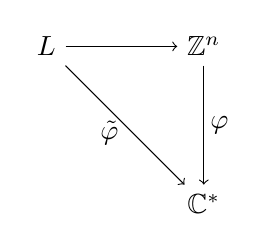
\begin{tikzpicture}
	\node(L) at (0,2) {$L$};
	\node(Z) at (2,2) {$\Z^n$};
	\node(C) at (2,0) {$\C^*$};
	\draw[->] (L) to (Z);
	\draw[->] (Z) to (C);
	\draw[->] (L) to (C);
	\node at (2.2,1) {$\varphi$};
	\node at (.8,.9) {$\tilde{\varphi}$};
	\end{tikzpicture}}
	\end{center}
	Recall that $Hom(\Z^n,\C^*)\simeq(\C^*)^n$, 
	and so we have 
	$$0\to Hom(A,\C^*)\to(\C^*)^n\to
	Hom(L,\C^*)\to0 $$

	{\scriptsize{\noindent\textbf{Example:} 
	Let $L\subseteq\Z^3$ be given by $(1,1,1)
	\Z+(1,3,5)\Z$. i.e. the integer 
	scaled ``lines'' from the two ``lines'' (which in 
	$\Z^3$ consist only of the lattice points 
	that coincide with the line in continuous space) 
	in $\Z^3$, one that is the diagonal through 
	the point (1,1,1), the other of which goes through 
	(1,3,5) with a slope of $1/\sqrt{35}$, $3/\sqrt{35}$, 
	and $5/\sqrt{35}$ in the $x$, $y$, 
	and $z$-directions respectively.\\
	Then $A=cok(L\hookrightarrow\Z^3)=\Z^3/L$. 
	Now, to get a better understanding of $A$, we can look at 
	this as an iterated quotient: first, we see that the 
	line $(1,1,1)\Z$ induces an equivalence of 
	values along that line in 3-space. 

	and so $A$ is isomorphic to $\Z\oplus\Z/2\Z$. 
	}}

	\noindent Now, since $(\C^*)^n$ acts on $\C^n$ and 
	$Hom(A,\C^*)$ is a subgroup of $(\C^*)^n$, 
	then $$Hom(A,\C^*)\circlearrowright\C^n.$$ 

	{\scriptsize{\noindent\textbf{Example:} 
	Recall: $Hom(\Z^3,\C^*)\simeq(\C^*)^3$, 
	and we have $$(\C^*)^3\to Hom(L,\C^*)\to0.$$ So: 
	\\
	\begin{minipage}{0.3\textwidth}
	\resizebox{0.9\textwidth}{!}{
	\begin{tikzpicture}
		\node (0) at (0,2) {0};
		\node (L) at (2,2) {$L$};
		\node (Z) at (4,2) {$\Z^3$};
		\node (C) at (4,0) {$\C^*$};
		\draw[->] (0) to (L);
		\draw[->] (L) to (Z);
		\draw[->] (L) to (C);
		\draw[->] (Z) to (C);
	 	\node at (2.8,.9) {$\tilde{\varphi}$};
	 	\node at (4.2,1) {$\varphi$};
	\end{tikzpicture}
	}
	\end{minipage}~
	\begin{minipage}{0.65\textwidth}
	Given $\sigma\in\C^*$, want to look at its 
	preimage in $L$. This gives us the pullback map 
	$\tilde{\phi}$ for any $\phi\in Hom(\Z^3,\C^*)$. 
	\\ So $(1,1,1)\Z+(1,3,5)\Z\hookrightarrow
	\Z^3\stackrel{\varphi}{\to}\C^*$. And, since 
	any function can be defined in terms of its values on the 
	three bases, this can be written: \\
	Given $\big(\varphi(1,0,0),\varphi(0,1,0),\varphi(0,0,1)\big)
	\in(\C^*)^3$, want its image in $(\C^*)^3\to
	Hom(A,\Z)$. 
	\end{minipage}
	}}
	Then $Hom(A,\C^*)$ is the kernel of the map 
	$(\C^*)^3\to Hom(L, \C^*)$, which we can 
	now compute, since we know how the map itself looks, as 
	in the example above. 

	Then write the action of $Hom(A,\C^*)$ on 
	$\C^3$ as an action on $\C[x_1,...,x_n]$, 
	and take the subring 
	$$S^0\subseteq\C[x_1,...,x_n]$$ 
	of invariants w.r.t. the action of $Hom(A,\C^*)$. 

	Thus we have a map: 
	$$0\to I\to\C[x_1,...,x_n]\to S^0\to0$$
	where this $I$ is the ideal that corresponds to the 
	kernel of the map. 

	Then $I$ induces a variety in $\C^3$ given by 
	$$Spec\left(\C^n//_0Hom(A,\C^*)\right)$$

	So the question now is: what does this variety do? 
	\subsection{Review}
	The procedure we have now can be summarized as follows: 
	Given a lattice $L$, we can form a short exact sequence: 
	$$0\to L\to\Z^n\to A\to0$$
	and follow the steps below to obtain a variety 
	$X(L)\subset\C^m$, usually denoted $Spec(
	\C[x_1,...,x_n]^G)$ where $G=Hom(A,\C^*)$. 
	\begin{enumerate}
		\item $0\to L\to\Z^n\to A\to0$
		\item Apply $Hom$ functor: 
		$$0\to Hom(A,\C^*)\to\Z^n
		\C^*)\simeq (\C^*)^n$$
		\item Recall $(\C^*)^n$ acts on 
		$\C^n$, so $G=Hom(A,\C^*)^n$ 
		acts on $\C^n$, as it is a subgroup 
		of $(\C^*)^n$ (as shown by the short 
		exact sequence from prev step)
		\item Find the invariant ring $\C
		[x_1,...x,_n]^G=\{f(x_1,...x_n):g\circ f=
		f~\forall g\in G\}$ and can see that this is 
		a finitely generated ring, so have a finite 
		set of monomials $\overline{x}^{I_1},...,
		\overline{x}^{I_m}$ s.t. 
		$$\C[x_1,...,x_n]^G=
		\C[\vec{x}^{I_1},...,\vec{x}^{I_m}]$$ 
		(Here there are relations between the 
		$\vec{x}^I$ terms)
		\item Now can take the kernel $I$ of the map 
		$\C[x_1,...x_n]\to\C
		[\vec{x}^{I_1},...\vec{x}^{I_m}]$ 
		to form a short exact sequence: 
		$$0\to I\to\C[z_1,...z_n]\to
		\C[\vec{x}^{I_1},...\vec{x}^{I_m}]$$
		and this ideal $I$ cna be generated by a 
		finite number of polynomials $$I=\langle 
		g_1(z_1,...,z_m),...,g_k(z_1,...,z_m)\rangle$$
		\item Take the zero set associated to $I$: 
		$$V(I) = \{(z_1,...z_m)\in\C^m: 
		g_i(\vec{z})=0~\forall i\}$$
	\end{enumerate}


	\section{Another approach}
	Let $(S,+)$ be an abelian semigroup. Then one can associate 
	a ring to it as follows: $$\C[S]=\C
	[x^s: s\in S]$$ where we define $x^s\cdot x^{\tilde{s}}=
	x^{s+\tilde{s}}$ for all $s,\tilde{s}\in S$. Suppose (
	for well-definedness) that $(S,+)\subset(\ {N},+)$, 
	and further suppose that $S$ is finitely generated. i.e. 
	$S=\langle s_1,...,s_m\rangle$. Then 
	$$\C[S]=\C[s_1,...s_m]$$ where the 
	$s_i$ might not be independent of each other. 
	Then, taking the map from $\C[w_1,...,w_m]$, 
	the polynomial ring on $m$ \emph{independent} variables 
	to $\C[s_1,...,s_m]$ by $w_i\to s_i$, note that, 
	as there are possible relations between the $s_i$, this 
	induces a kernel, and so we have a short exact sequence: 
	$$0\to I_S\to\C[w_1,...,w_m]\to\C[ s_1,...,s_m]$$ 
	and the zero set of this ideal forms the 
	variety: $$Spec(\C[S])=V(I_S)\subset\C^m$$
	Claim: Given $0\to L\to\Z^n\to A\to0$, then 
	$$Spec\left(\C[x_1,...x_m]^{Hom(A,\C^*)}\right)
	\simeq Spec(\C[L\cap\N^n])$$
	Now, given the lattice and associated short exact sequence, 
	can define a \textbf{multigrading} in $\C[x_1,...x_n]$ 
	e.g. for $L=\Z^2\subset\Z^3$, 
	$$\begin{array}{rcccccl}
		0\to&\Z^2&\to&\Z^3&\to&\Z&\to0\\
		&(1,0,-1)&&(1,0,0)&\to&1&\\
		&(1,-1,0)&&(0,1,0)&\to&1&\\
		&(0,1,-1)&&(0,0,1)&\to&1&
	\end{array}$$
	Then $deg(\vec{x}^{(a_1,a_2,a_3)}=\varphi(a_1,a_2,a_3)
	=a_1\varphi(1,0,0)+a_2\varphi(0,1,0)+a_3\varphi(0,0,1)$. 
	This gives the traditional grading, but we could define 
	the map differently. e.g.
	$$\begin{array}{cccl}
		\Z^2&\to&\Z&\to0\\
		(1,0)&\to&1&\\
		(0,1)&\to&-1&
	\end{array}$$
	Note that a homogeneous polynomial with this grading would 
	look something like $x^3+y^2x^5$. Note, we could even have 
	had the map $\Z^2\to\Z_3\to0$, where 
	$x^2=x^{2+3n}$ for all $n\in\Z$

	Claim: $f\in\C[x_1,...,x_n]^G$ iff $deg_A(f)=0$. 

	So $L$ are the elements ``of degree 0'' with respect to the 
	multigrading. 
	\\\noindent\textbf{Example}:\\
		$L=\{(n_1,n_2):n_1+n_2=3k, k\in\Z\}$, then 
		we have the ses: $$0\to L\to\Z^2\to A\to0$$
		where $A\simeq\Z/3\Z$, and the 
		multigrading on the ring: 
		$$\C[x_1,x_2]\to\Z_3\to0$$
		s.t. $deg_A(x_1)=w$, $deg_A(x_2)=w$, and $w^3=1$. 
		So the homogeneous monomials of degree 0 are: 
		$x_1^3, x_1^2x_2, x_1x_2^2, x_2^3$.

	\section{Generalizing for the cases with singularities}
		We now have a procedure (2 really) whereby, given 
		a lattice, one can obtain a toric variety associated 
		to that lattice. It turns out that very often this 
		variety is trivial(a point), and so we need to 
		introduce some new machinery to identify in which 
		cases this occurs, and also to introduce a modification 
		which will produce varieties that are not trivial.


		\noindent\textbf{Theorem}: Let $S=\C[x_1,...,x_n]$. 
		TFAE:
		\begin{enumerate}
		\item $\exists a\in A$ such that 
		$$S_a:=\{x^{I_1}\in S\mid: deg(x^{I_1})=a\}$$ 
		is a finite dimensional vector space
		\item $S_0\simeq\C$
		\item $L\cap\N^n=\{0\}$. 
		\end{enumerate}

		\noindent\textbf{Definition}: $A$ is a \textbf{positive grading} 
		if $S_0\simeq\C$. 

		\noindent\textbf{Example}: $\Z^2\to\Z\to0$ by 
		$x\mapsto1$, $y\mapsto-1$, then $L=\{(n,m):n-m=0\}$ 

		\noindent\textbf{Theorem}: If $A$ is a positive grading, 
		then $L\cap\N^n=\{0\}$ so $\C[0]=\C$ 
		and $Spec(\C)=$ point.

		Hence the need for a generalization. It turns out that the idea 
		of multigrading admits precisely the tool needed to produce 
		nontrivial varieties. 

		Note: $S_{na}\times S_{ma}=S_{(m+n)a}$ gives the infinite 
		direct sum $$\bigoplus\limits_{n\ge0}S_{na}$$ a ring structure, 
		and so can set $$S_{(a)}=\bigoplus\limits_{n\ge0}S_{na}$$ 
		a finitely generated ring, and so we have a map 
		$$\C[z_1,...z_m]\to S_{(a)},~~\text{ by }~~
		z_i\mapsto x^{I_i}$$
		and so there is an ideal associated to this map: 
		$$0\to I\to\C[z_1,...,z_m]\to S_{(a)}$$
		and the zero set of $I$ is a variety!(?) 

		Another way of seeing this is to see $S_{(a)}=
		\C[x^{I_1},...x^{I_m}]$ where the $x^{I_i}$ are 
		the generators, and so we have a map from an open set 
		$x_1,...,x_n\in(\C^*)^n\mapsto(\vec{x}^{I_1},...x^{I_m})$ 
		which is contained in some open $U\subset\CP^m$ and can 
		take the closure of the image. 

		\noindent\textbf{Theorem}: There is a map $Proj(S_{(a)})\to
		Spec(S_{(0)})$. 
	\subsection{When do we have a compact variety}
		\noindent\textbf{Remark}: $\CP^n=\C^{n+1}/\sim$ the standard equivalence class 
		$\vec{x}\sim\vec{y}$ iff $\exists s\in\C^*$ s.t. $\vec{x}=s\vec{y}$. 
		And $\CP^n$ is a smooth variety. 
		
		One consequence of this is as follows: let $f(x_1,...,x_{n+1})$ 
		be a polynomial s.t. $\forall s\in\C^*$, $f(sx_1,...sx_{n+1})=
		s^mf(\vec{x})$. Then if $\vec{p}\sim\vec{q}$ and $f(\vec{p})=0$, 
		then $f(\vec{q})=0$ also, so it is well-defined to say 
		$$f([p])=0~~\text{ for }[p]\in\CP^n$$ and say that 
		$f$ is \textbf{homogeneous}. 
		Further, let $I\subset\C[x_1,...,x_{n+1}]$. 
		Recall that every ideal has a finite number of generators 
		$$I=\langle f_1,...,f_m\rangle$$
		Then if $f_i$ is homogeneous for all $i$, then $I$ defines a 
		variety in $\CP^n$ and denote it 
		$$Proj\left(\frac{\C[x_1,...x_n]}{I}\right)$$
		The difference between this and the other variety 
		construction is (intuitively): 
		$Proj(S/I)$ is compact, whereas $Spec(S/I)$ is not always. 

		$Proj$ is a section, and so only well-defined if $I$ is 
		homogeneous. 

		\noindent\textbf{Remark}: $f(x_1,...,x_{n+1})$ is homogeneous 
		iff $f(x_1,...x_{n+1})=\sum\limits_{I\in\N_{n+1}}C_Ix^I$ where 
		$deg(x^I)$ is constant over $I$. However, we have multigrading 
		machinery, so can define a more general $\CP^n$ for such 
		gradings. 

		In conclusion, given a homogeneous ideal $I$, we have a 
		compact variety in some $\CP^n$ which is denoted $Proj(S/I)$. 

	\subsection{Review}
		We have the ses $0\to L\to\Z^{n+1}\to A\to0$, then if 
		$L\cap\N^{n+1}=\{0\}$ or equivalently if $S_0=\C$, then 
		$$Spec\left(\frac{S}{I}\right)=pt$$
		However, if we fix $a\in A$, can construct a ring 
		$$S_{(a)}=\bigoplus\limits_n S_{(na)}$$ and an 
		exact sequence $$0\to I_{(a)}\to\C[z_1,...,z_m]\to S_{(a)}\to0$$ 
		and the variety 
		$$Proj(S_{(a)})=Proj\left(\frac{\C[z_1,...,z_m]}{I_{(a)}}\right)$$

		\noindent\textbf{Question}: How do we know if $I_{(a)}$ is 
		homogeneous? Answer: look at the $I_i$ for $S_{(a)}\simeq
		\C[\vec{x}^{I_1},...,\vec{x}^{I_m}]$. 

		\noindent\textbf{Example}: Take the quiver below, and let \\
		\begin{minipage}{0.65\textwidth}
		$A=\left\{(\theta_1,\theta_2)\in\Z^{Q_0}\mid\theta_1+\theta_2=0\right\}$. 
		Consider $\Z^{Q_1}\to A$ by $inc$, the inclusion map. 
		Then $inc(1,1)=(-2,2)$.  Let $Cir(Q):=ker(inc)$. Then in 
		our case, this will be 
		$$ (1,0)\mapsto(-1,1),~~~ (0,1)\mapsto(-1,1)$$
		and so $Cir(Q)=\{(n,-n):n\in\Z\}=(1,-1)\Z$.
		\end{minipage}~\begin{minipage}{0.3\textwidth}
			\resizebox{0.9\textwidth}{!}{
				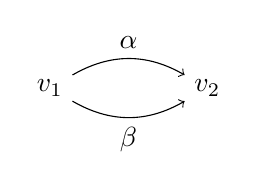
\begin{tikzpicture}
					\node(v1) at (0,0) {$v_1$};
					\node(v2) at (2,0) {$v_2$};
					\draw[->, bend left]  (v1) to node[midway, above] {$\alpha$} (v2);
					\draw[->, bend right] (v1) to node[midway, below] {$\beta$} (v2);
				\end{tikzpicture}
			}
		\end{minipage}
		Recall: $0\to Hom(A,\C^*)\to Hom(\Z^2,\C^*)\to Hom(L,\C^*)\to0$
		and $G= Hom(A,\C^*)\subset(C^*)^2$. Want to know how this containment 
		works. Let $t_1=Im(1,0)$, $t_2=Im(0,1)$. Then 
		$$Hom(\Z^2,\C^*)\to Hom(L,\C^*)~\text{ by }
		(t_1,t_2)\mapsto t_1^2t_2^{-2}$$
		and so $G=\{(t_1,t_2):t_1^2t_2^{-2}=1\}=
		\{(t_1,t_2)\in(\C^*)^2:t_1^2=t_2^2\}=\{(t_1,t_2)\in(\C^*)^2:t_1=\pm t_2\}$

	\section{Polytope to Variety}
	Let $\Lambda\subset\R^n$ be a lattice, i.e. $\Lambda\simeq\Z^n$. 
	We say $P$ is a \textbf{lattice polytope} if every vertex of $P$ 
	belongs to $\Lambda$. 

	Let $P$ be a lattice polytope of dimension $n-d$. Will next describe 
	the mechanism for producing a variety $X_P$. 

	\begin{enumerate}
		\item $\forall$ lattice polytope $P$ can be written 
		$$P=\{\vec{x}\in\R^{n-d}:~\vec{v}_i\cdot\vec{x}\ge-w_i\}$$
		e.g. 
	\item Given $\vec{v}_i\in\R^{n-d}$, $\vec{w}\in\R^n$, define a map 
		$$\varphi:\R^{n-d}\to\R^n~\text{ by } x\mapsto(
		\vec{v}_1\cdot\vec{x},...,\vec{v}_n\cdot\vec{x})$$
		Note that $V:=\varphi(\R^{n-d})$ is an $(n-d)$-dimensional 
		vector subspace and $\varphi(P)\simeq P$ is given by 
		$$V\cap\R^n_{\ge-w_i}$$
		Let $L:=V\cap\Z^n\subset\R^n$. 
		and so have $$0\to L\to\Z^n\to A\to0$$ and an 
		$\vec{a}\in A$ s.t. $\vec{a}=im(\vec{w})$. 
		e.g. 
	\item Recall previous discussion with $\C^n//_a Hom(A,\C^*)$. 
	\item Explicitly find the ideal associated to $\C^n//_aHom(A,\C^*)$. 
	This needs the same generators of the ring $S_{(a)}=\oplus S_{n\vec{a}}$
	where $S_{d\vec{a}}=\{\vec{m}\in\C[z_1,...,z_m]:~deg_A(\vec{m})=\vec{a}d\}$. 
	\end{enumerate}
	So given a polytope $P$, can find a complex variety $X_p$, and given 
	a projective toric variety, the polytope is unique up to scaling and 
	$GL(n,\Z)$. 
\end{document}
